\documentclass[sigconf]{acmart}

\usepackage[english]{babel}
\usepackage{blindtext}
\usepackage{subfig}

% Copyright
\renewcommand\footnotetextcopyrightpermission[1]{} % removes footnote with conference info
\setcopyright{none}
%\setcopyright{acmcopyright}
%\setcopyright{acmlicensed}
%\setcopyright{rightsretained}
%\setcopyright{usgov}
%\setcopyright{usgovmixed}
%\setcopyright{cagov}
%\setcopyright{cagovmixed}

\settopmatter{printacmref=false, printccs=false, printfolios=true}

% DOI
\acmDOI{}

% ISBN
\acmISBN{}

%Conference
%\acmConference[Submitted for review to SIGCOMM]{}
%\acmYear{2018}
%\copyrightyear{}

%% {} with no args suppresses printing of the price
\acmPrice{}


\begin{document}
\title{DE-CIX Outage/Atlas Coverage/Impact Extrapolation}

%\titlenote{Produces the permission block, and copyright information}
%\subtitle{Extended Abstract}

% \author{Paper \# XXX, XXX pages}
\author{Ann Author}
% \authornote{Note}
% \orcid{1234-5678-9012}
\affiliation{%
  \institution{Affiliation}
  \streetaddress{Address}
  \city{City} 
  \state{State} 
  \postcode{Zipcode}
}
\email{email@domain.com}

% The default list of authors is too long for headers}
\renewcommand{\shortauthors}{Ann Author, et al}

\begin{abstract}
%"Five sentences"
%1: Motivation:
%2: Problem statement:
%3: Approach:
%4: Results:
%5: Conclusions:

Outages are a natural part of the operational reality of the Internet. Their
impact is often viewed through the lens of media reporting, reporting from the
affect organisations themselves, and user reports. Are these sufficient for
understanding the impact of an outage? Researchers may use platforms such as
RIPE Atlas to understand traffic behaviour around configuration changes, and
outages are highly likely to prompt notable rerouting events. Is RIPE Atlas, or
are other data sources, capable of modelling a resulting outage to help us
understand what the real impact is?
\end{abstract}

\maketitle

\section{Introduction}

% 1: Motivation. Why is this important?
Localised outages are an inevitable occurrence in large-scale infrastructure
projects such as the Internet. Understanding their impact is nontrivial:
Internet service providers are generally unlikely to advertise to their users
when their performance is degraded, and localised user reports do not offer a
complete picture.

% 2: What is the focus of this paper?
Measurement platforms, such as RIPE Atlas, provide greater visibility into
network conditions, but what metrics and data sources are available to help us
extrapolate a more complete picture of an outage's impact? 

% 3: What do we show? "In this paper, ..."
In this paper, we examine the impact of a recent power outage at one of the
locations operated by DE-CIX, a large European Internet exchange point. We
correlate [various things: RIPE Atlas measurements, PCH BGP updates, lists of
peering partners published by DE-CIX, Romain's Internet Health Reports] to
understand what traffic was impacted, and how.

% 4: How is this novel?
This approach is novel in terms of [...]

% 5: 
The remainder of this paper is structured as follows: [...]

% --------------------------------------------------------------------------
\section{Related Work}

~\cite{labs:damage:2015, labs:damage:2018}


% --------------------------------------------------------------------------
\section{DE-CIX FRA Power Outage}

In this section, we discuss the event in question, and the public data sources
available to us.

Two distinct power failures occurred on the night of 9th and 10th of April 2018
at one of DE-CIX's locations, ``DE-CIX6/FRA5''~\cite{tweet:decix-1, tweet:decix-2}.
Their public traffic stats are shown in Figure~\ref{i:decix:public}.

\begin{figure}[tp]
  \centering
  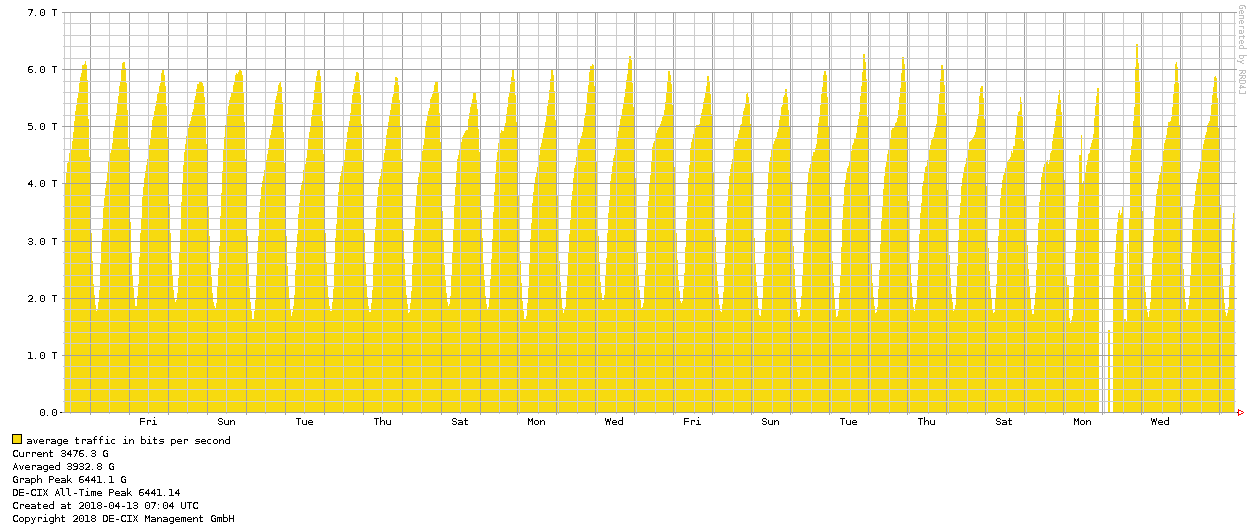
\includegraphics[width=1\columnwidth]{images/traffic_FRA-1month-1170-400.png}
  \caption{Public DE-CIX traffic graph}
  \label{i:decix:public}
\end{figure}

DE-CIX also releases public BGP data via PCH. Table snapshots are released once
every 24 hours, and those are likely to show any before/after state changes but
not the outage itself. BGP update streams however are released continuously and
allow us to visualise BGP activity at DE-CIX's route collectors. The timeseries
of updates is show in Figures~\ref{i:decix-pch-linear}
and~\ref{i:decix-pch-log}.

\begin{figure}[tp]
\centering
\subfloat[decix PCH]{
  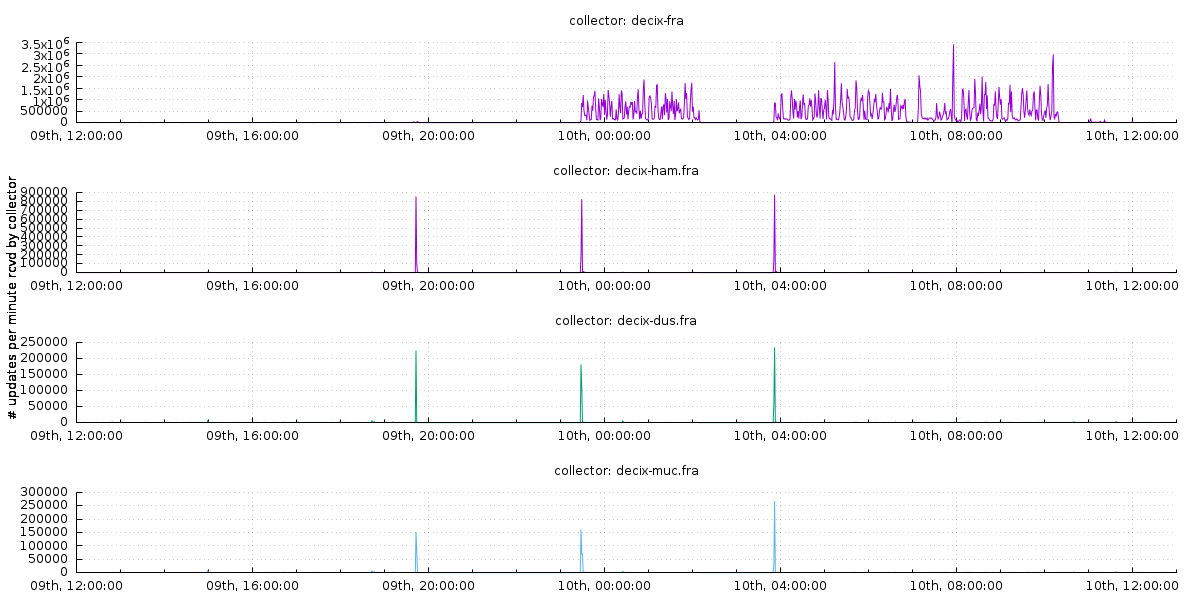
\includegraphics[width=1\columnwidth]{images/decix-linear.png}
  \label{i:decix-pch-linear}
}

\subfloat[decix PCH (logscale y)]{
  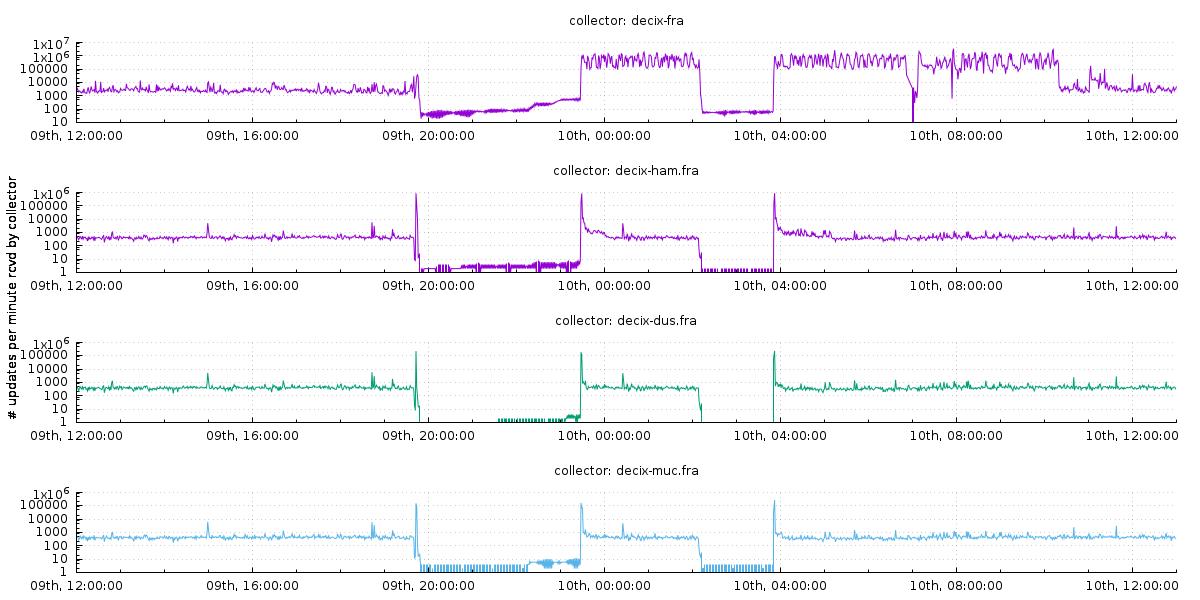
\includegraphics[width=1\columnwidth]{images/decix.png}
  \label{i:decix-pch-log}
}
\end{figure}


\textit{What other data sources do we have, and how can we leverage those? What
techniques and public data sources are available?}

IXPs list their members to encourage other networks to join. DE-CIX
provides machine-readable lists of their members at various locations:~\cite{members-fra,
members-dus, members-ham, members-muc}.

\textit{Routing data: PCH~\cite{} provides archives of route collector data. DE-CIX has four:}

\begin{itemize}
\item DECIX-FRA: route-collector.fra.pch.net
\item DECIX-DUS: route-collector.decix-dus.fra.pch.net
\item DECIX-HAM: route-collector.decix-ham.fra.pch.net
\item DECIX-MUC: route-collector.decix-muc.fra.pch.net
\end{itemize}

\textit{What is the overlap of the membership lists and Atlas probe deployment?
Can we say anything about the `goodness' of measurements in
Section~\ref{s:impact} using only this?}

\textit{Can we use the prefixes specifically in these tables to narrow the
search space for effects in Atlas measurements? Can we identify effects on
containing prefixes in other tables from other sources (RIS?)}

% ---------------------------------------------------------------------------
\section{How is traffic impacted?}
\label{s:impact}

\textit{Figure~\ref{i:decix:atlas} demonstrates the impact to Atlas
traceroutes. [Detail: which measurements, where the data is, how those traces
were selected, what the shortfalls of that process are]}

\begin{figure}[tp]
  \centering
  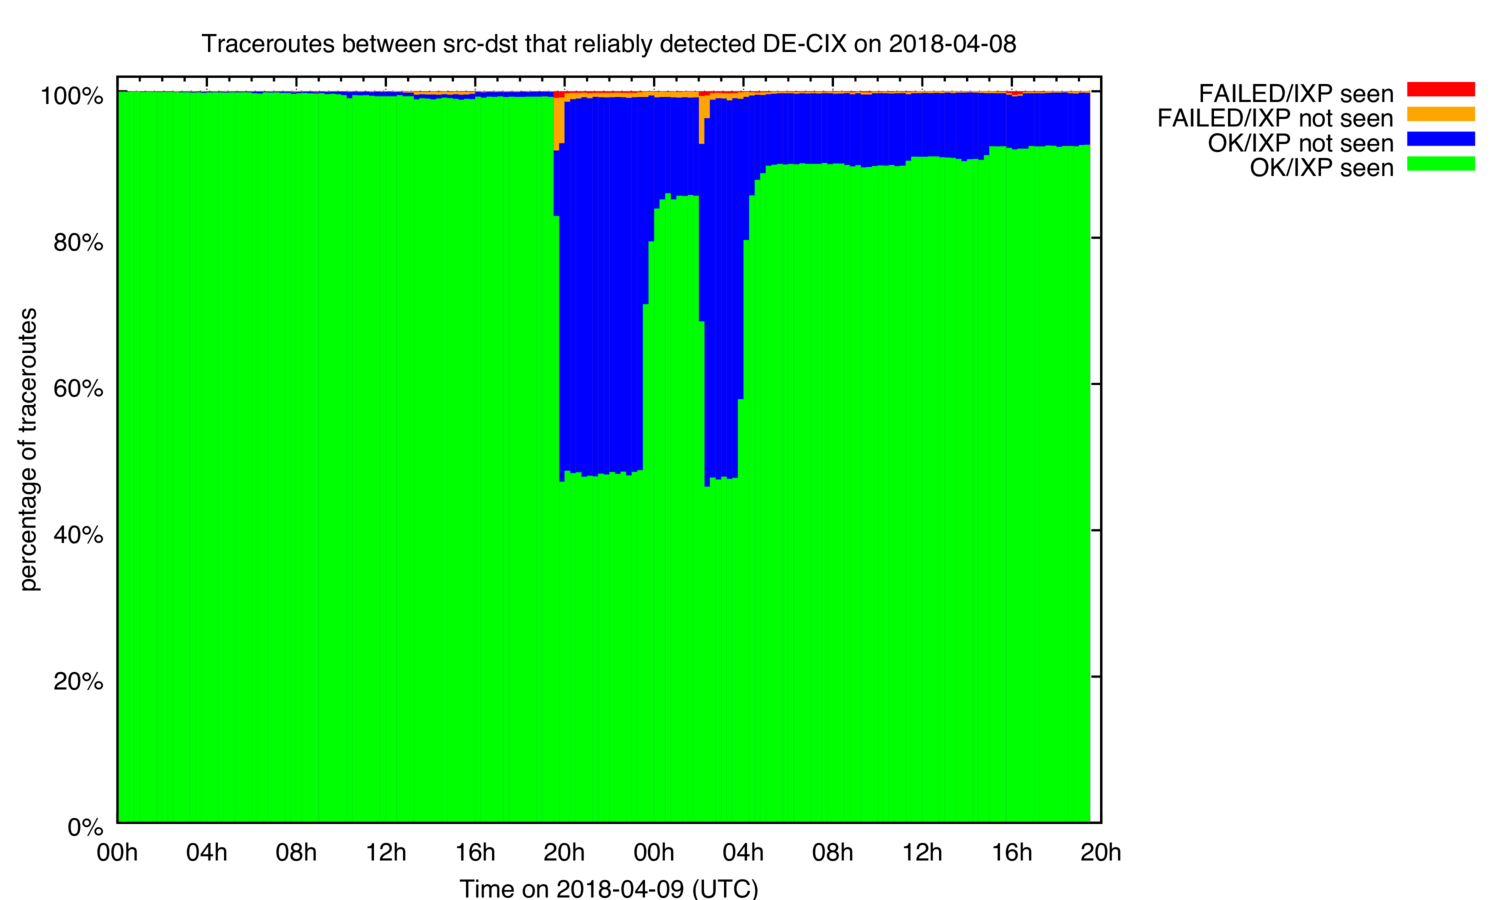
\includegraphics[width=1\columnwidth]{images/decix-2018-04-09-goodput.png}
  \caption{probe reachability as observed by active traceroutes}
  \label{i:decix:atlas}
\end{figure}

% ---------------------------------------------------------------------------
\section{How is the network graph affected?}

Figures~\ref{i:ihr-1},~\ref{i:ihr-2},~\ref{i:ihr-3}


\textit{How does this affect latencies between probes? How does this affect
latencies to content? Does it affect latencies to content?}

\begin{figure}[tp]
\centering
\subfloat[ihr-1]{
  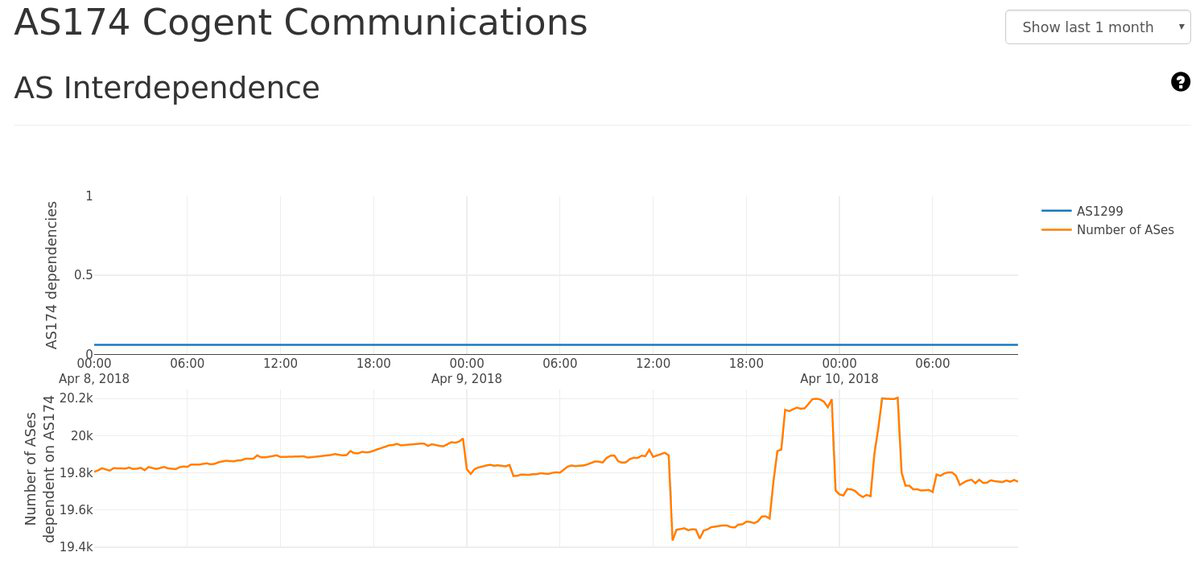
\includegraphics[width=1\columnwidth]{images/ihr-1.png}
  \label{i:ihr-1}
}

\subfloat[ihr-2]{
  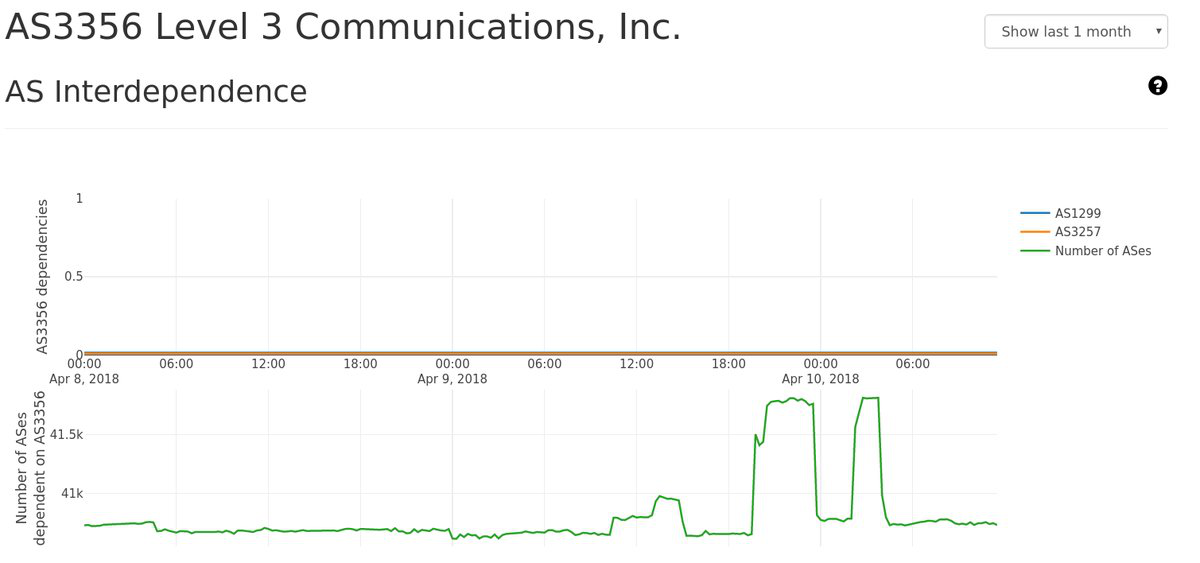
\includegraphics[width=1\columnwidth]{images/ihr-2.png}
  \label{i:ihr-2}
}

\subfloat[ihr-3]{
  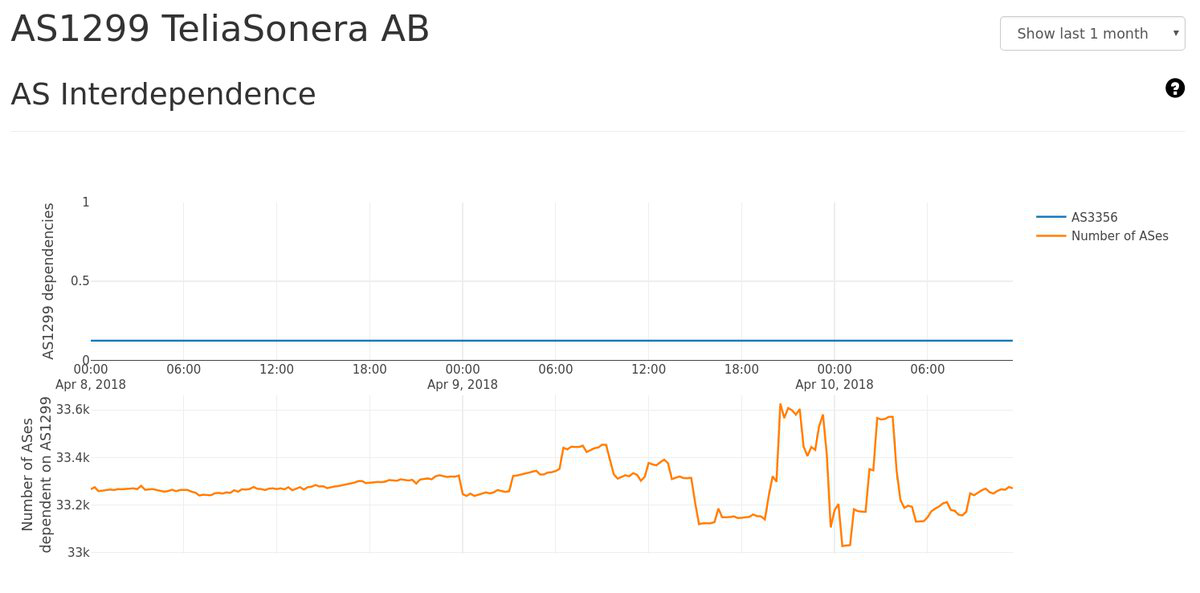
\includegraphics[width=1\columnwidth]{images/ihr-3.png}
  \label{i:ihr-3}
}

\subfloat[ihr-4]{
  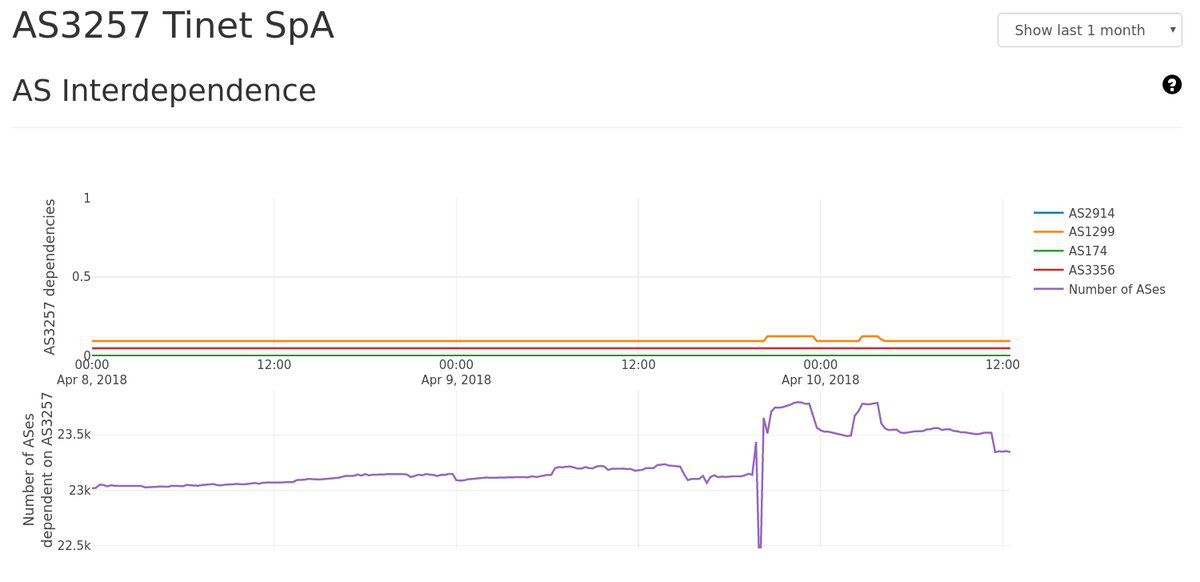
\includegraphics[width=1\columnwidth]{images/ihr-4.png}
  \label{i:ihr-4}
}

\end{figure}


% ---------------------------------------------------------------------------
\section{Conclusion}

\textit{Why are these interesting? is this an interesting side effect of the outage? ``Who cares?''}

\textit{Conclusions?}




\bibliographystyle{ACM-Reference-Format}
\bibliography{paper}

\end{document}
